%
% Draft  document curv.tex
% Predicting intrinsic radius of fibre curvature from follicle curvature
%
 
\documentclass[titlepage]{article}  % Latex2e
\usepackage{graphicx,lscape,subfigure}
\usepackage{bm}
\usepackage{textcomp}
 

\title{ Can we predict intrinsic fibre curvature from follicle curvature score?}
\author{Neville Jackson and Jim Watts}
\date{18 May 2016} 

 
\begin{document} 
 
\maketitle      
\tableofcontents

\clearpage
\section{Introduction} 
The intrinsic curvature of wool fibres has been shown to  be one of the basic fibre metrics involved in bulk compressional properties, handle and product quality (Swan(1993)~\cite{swan:93}. Its measurement using {\em Laserscan} or {\em OFDA} technology is available today, but was not available when many of the classic Merino genetics datasets were collected.It is therefore of some importance to see whether intrinsic fibre curvature could be predicted from the follicle curvature scores developed by Nay and Jackson(1973)~\cite{nayj:73} Some of the classic Merino genetics datasets do have follicle curvature score, so predicting fibre curvature from follicle curvature would enhance these datasets and the genetic information obtained therefrom.


\section{Methods}
\subsection{Measurement of fibre curvature in follicles}
 The follicle curvature score diagrams of Nay and Jackson(1973)~\cite{nayj:73} were used to obtain data on fibre curvatures corresponding to each follicle curvature score grade.  The diagrram for each follicle curvature score grade consists of a drawing of follicles as seen in a thick vertical skin section.  The diagram is 3-dimensional, so that some follicles are seen at right angles to the plane of maximum curvature, while other follicles are seen at various orientations so that their maximum curvature is not displayed. 

It was decided to attempt to measure only those follicles showing maximum curvature, within each score grade diagram. Hopefully only follicles with the fibre suitably oriented would be measured by this procedure.

 Given that we wished to measure fibre (not follicle) curvature, it was decided to avoid the straight neck region of the follicles (where the fibre curvature could be constrained), and to also avoid the bulb region of the follicles ( where the keratinization which leads to fibre curvature has not yet occured). To this end, only the centre section of follicles was considered for measurement. The key assumption here is that the fibre is in a relaxed state in the centre follicle region and is thus displaying its intrinsic curvature.

The method for measurement of fibre curvature in vertical sections is illustrated in Figure~\ref{curvmeas}.

%\documentclass{article}
%\usepackage{graphicx,subfigure}
%\begin{document}

\begin{figure}[!h]
  \centering
   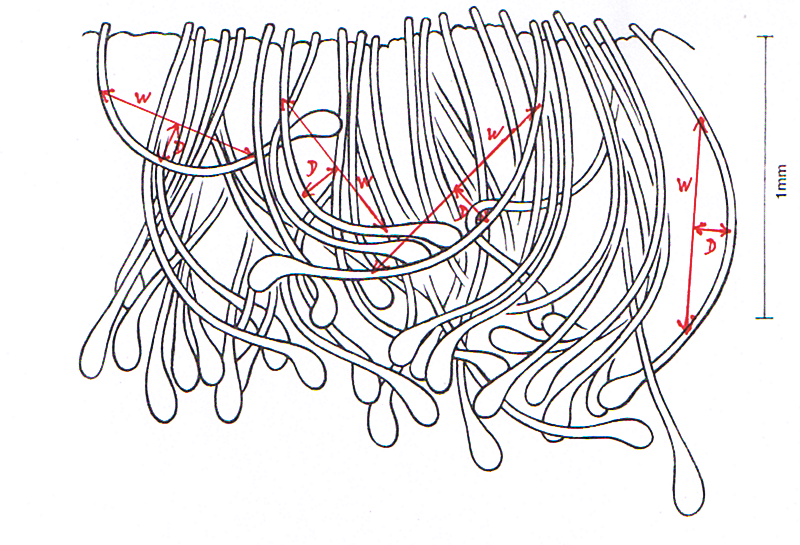
\includegraphics[width=0.9\textwidth]{curvmeas.png}
%  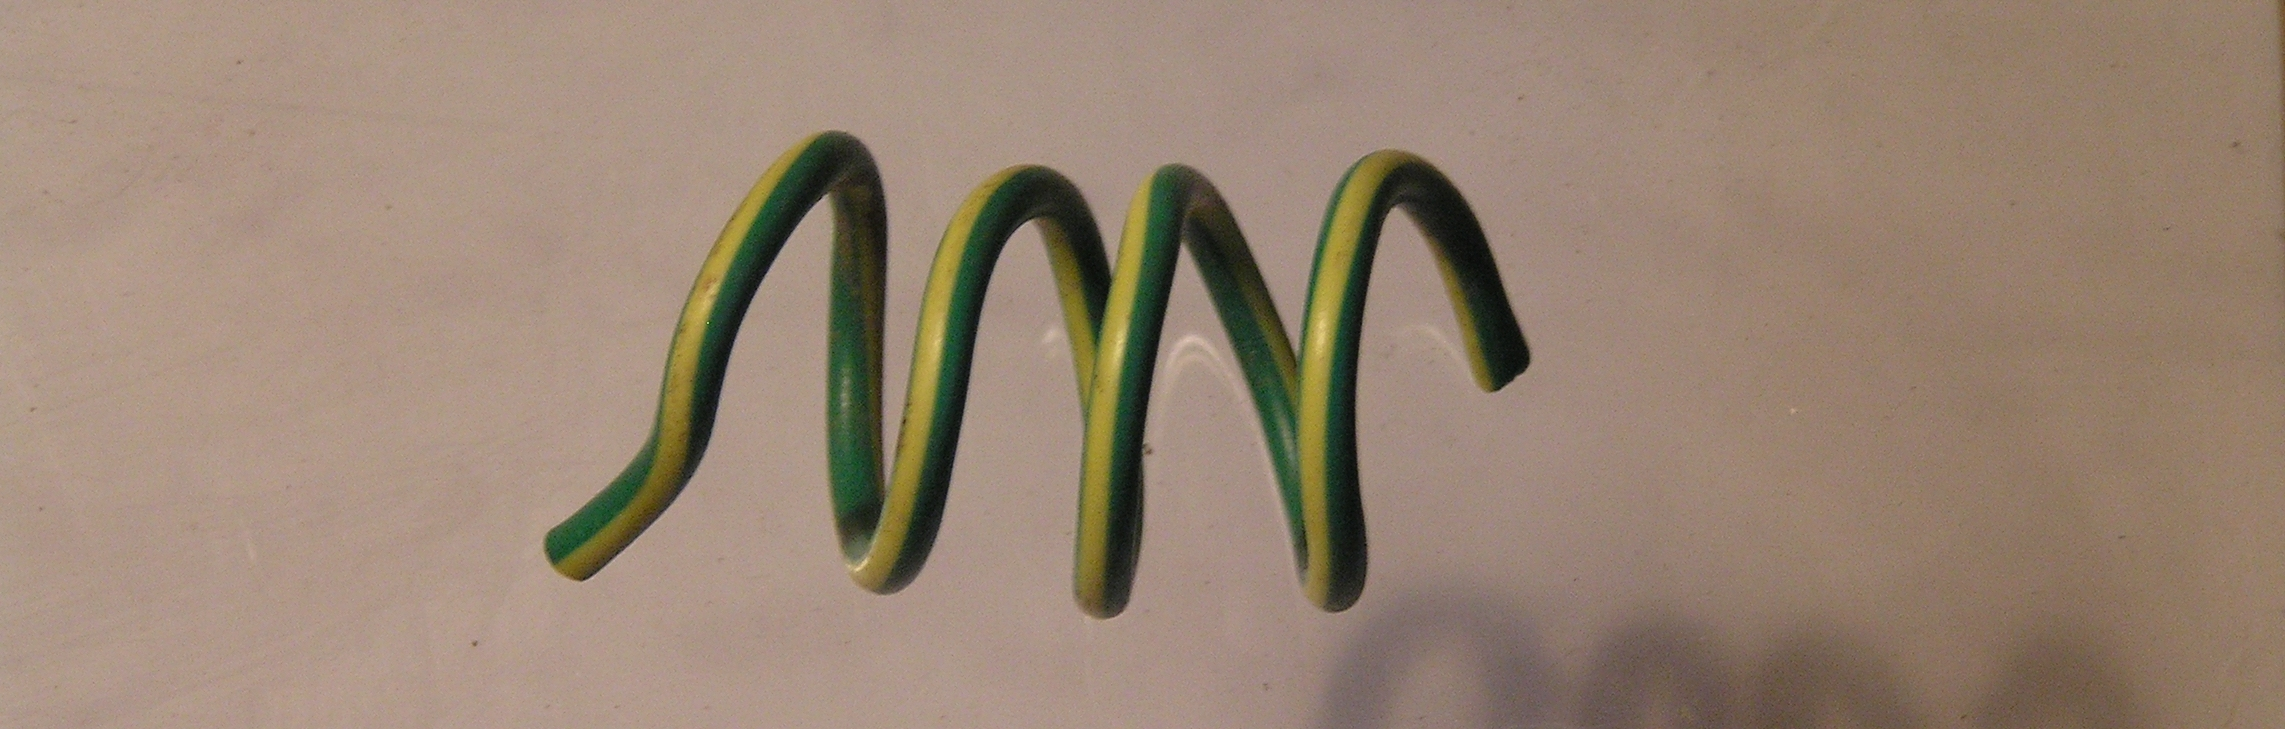
\includegraphics{fig1.png}
  \caption{Illustration of method of measurement of intrinsic radius of curvature of fibres in follicles in a vertical skin section}
  \label{curvmeas}
\end{figure}

%\end{document}



A curved section of follicle is chosen as indicated above, a chord of length $W$ is drawn across the curve, and a line perpendicular to the chord at its centre point is drawn and measured as $D$. The radius of curvature is given by

\begin{equation}
\label{r1}
R = \frac{D}{2} + \frac{W^{2}}{8 D}
\end{equation}
and is in units of mm, if the measuements of $W$ and $D$ are in mm.

An alternative formula used by Swan(1993)~\cite{swan:93} uses $a$ for $D$ and $b$ for $\frac{W}{2}$ and is written
\begin{equation}
\label{r2}
R = \frac{a^{2} + b^{2}}{2 a}
\end{equation}

Equations ~\ref{r1} and ~\ref{r2} are equivalent, they lead to exactly the same numerical value for radius.  These equations assume that the fibre arc is a circular arc, that is its radius of curvature is constant for all points along the arc. 

Curvature is obtained as the reciprocal of radius
\begin{equation}
\label{c1}
C = \frac{1}{R}
\end{equation}
and as obtained from equation~\ref{c1} above is in units of radians per mm.  The convention for wool industry reporting of fibre curvature (ie Laserscan or OFDA measurement) seems to be to use degrees per mm. Regardless of whether one uses degrees or radians per mm, what it represents is the angle subtended by an arc of a circle of length equal to 1 mm. This is readily seen from the formula for arc length $S$ given radius $R$ and angle $\theta$ in radians

\begin{equation}
\label{c2}
S = R \theta
\end{equation}
where on substituting $1$ mm for $S$ we get equation~\ref{c1}

If we want degrees per mm we multiply $C$ by the number of degrees in one radian ($180/\pi$).

Only between 6 and 8 fibre curvature measurements could be obtained from each follicle curvature score diagram

\subsection{Measurement of fibre curvature in the staple with OFDA-2000}
These measurements were performed in a commercial wool testing laboratory. A collection of 159 wool samples from 16 properties with known follicle curvature scores representing the full range of scores from 1 to 7 were tested. Results were reported as mean fibre curvature (degrees per mm), and standard deviation of fibre curvature.

Also available on these wools were crimp frequency (crimps /cm), mean fibre length (mm), fibre length to staple length ratio, follicle depth (mm), and follicle curvature score.

\subsection{Statistical analysis}
 Data were imported into the R statistical program~\cite{rprog:13} and analysed using the {\em odregress()} function fitting an orthogonal regression equation to predict fibre curvature from follicle curvature score. It was appropriate to predict fibre curvature ($C$) rather than intrinsic fibre radius ($R$) as this made the fitted regression equation linear and normalised the residuals. Orthogonal regression was used because both the predictor variable ( follicle curvature) and the predicted variable ( fibre curvature) were subject to measurement error.

The same anaalysis was applied to the in-follicle fibre curvature measurements and the OFDA in-staple fibre curvature measurements.


\section{Results}
\subsection{Fibre curvature in follicles}
The data for follicle curvature score and measured fibre radius in the follicle are shown in Figure~\ref{rawdata}.

%\documentclass{article}
%\usepackage{graphicx,subfigure}
%\begin{document}

\begin{figure}[!h]
  \centering
   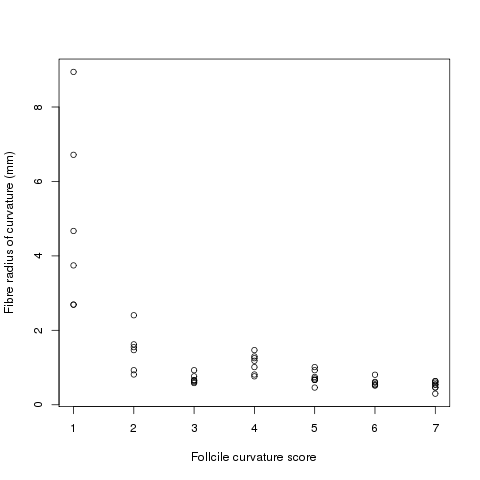
\includegraphics[width=0.9\textwidth]{fig2.png}
%  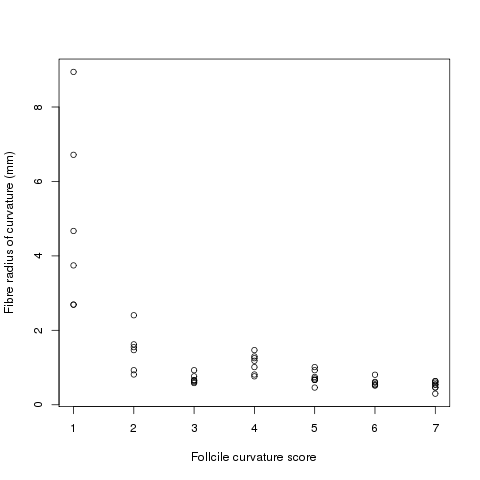
\includegraphics{fig2.png}
  \caption{Measured radius for a number of fibres from  vertical sections of given follicle curvature score}
  \label{rawdata}
\end{figure}

%\end{document}



The relationsjhip of follicle curvature score to measured fibre radius of curvature is clearly non-linear. It can be made linear by a reciprocal transformation from radius to curvature as in equation~\ref{c1}. The transformed data are shown in Figure~\ref{trandata}.

%\documentclass{article}
%\usepackage{graphicx,subfigure}
%\begin{document}

\begin{figure}[!h]
  \centering
   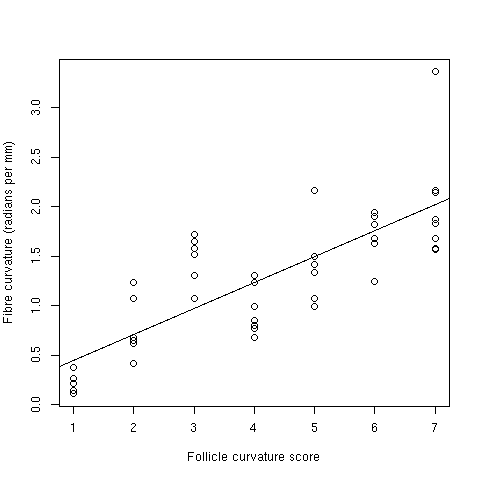
\includegraphics[width=0.9\textwidth]{fig3odr.png}
%  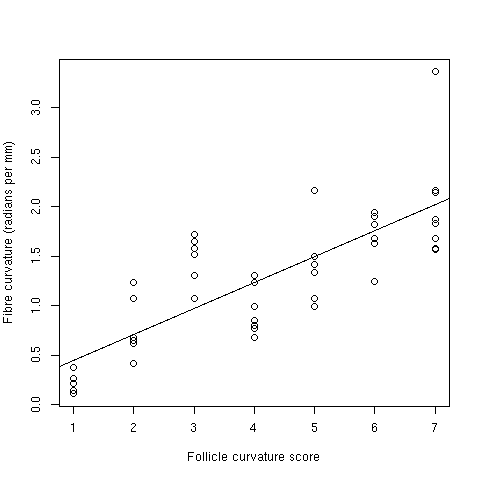
\includegraphics{fig3odr.png}
  \caption{Curvature obtained from the reciprocal transform of radius for number of fibres from  vertical sections of given follicle curvature score. The straight line is the fitted orthogonal regression equation.}
  \label{trandata}
\end{figure}

%\end{document}



 The relationship is now approximately linear, so that an orthogonal linear regression equation can be fitted to obtain a predictor equation. The fitted equation was

\begin{equation}
\label{eqn:in-follicle}
Y = 0.1840 + 0.2620 X
\end{equation}

where Y is Fibre curvature (in radians per mm) and X is follicle curvature score. The fitted equation is shown as the straight line on Figure~\ref{trandata}.
The follicle curvature score and measured fibre curvature  had a correlation  of $0.784$ and an analysis of variance showed that the regression on follicle curvature score was highly significant.

Using this equation the predicted fibre curvature for each follicle curvature score and the corresponding fibre radius is shown on Table~\ref{tab:pred}

%\documentclass{article}
%\usepackage{lscape}
%\begin{document}

\begin{table}[h]
\centering
\caption{Predicted values of intrinsic fibre radius of curvature, and intrinsic fibre curvature for each follicle curvature score}
\label{tab:pred}
\vspace{0.1in}
\begin{tabular}{p{0.8in}|p{0.8in}|p{0.8in}|p{0.8in}}  \hline
  Follicle curvature score & Predicted fibre curvature  & Predicted fibre curvature & Predicted fibre radius  \\ 
  (score) & (radians per mm) & (degrees per mm)&  (mm)  \\ \hline
 1  & 0.446 & 25.55 & 2.242 \\
 2  & 0.708 & 40.56 & 1.412 \\
 3  & 0.970 & 55.57 & 1.030 \\
 4  & 1.232 & 70.58 & 0.811 \\
 5  & 1.494 & 85.59 & 0.669 \\
 6  & 1.756 & 100.61 & 0.569 \\
 7  & 2.018 & 115.62 & 0.495 \\ \hline
\end{tabular}
\end{table}

%\end{document}

 
The predicted fibre curvatures in  degrees per mm in Table~\ref{tab:pred} are certainly in the range commonly observed for Merino sheep using Laserscan of OFDA techniques.

\subsection{Fibre curvature in the staple}
The data for follicle curvature score and OFDA measurement of fibre curvature in staples are shown in Figure~\ref{fig:ofdarads}, with the OFDA mean curvature converted to radians per mm. 

%\documentclass{article}
%\usepackage{graphicx,subfigure}
%\begin{document}

\begin{figure}[!h]
  \centering
   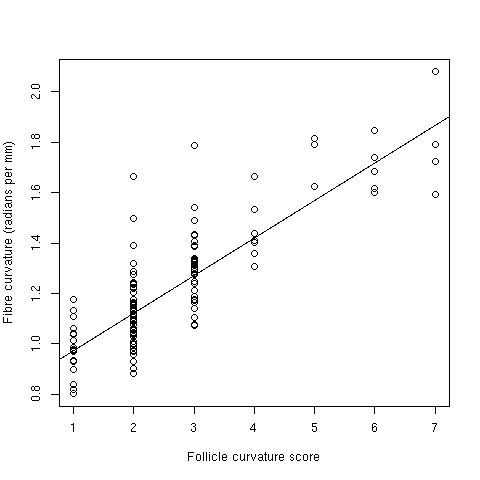
\includegraphics[width=0.9\textwidth]{ofdarads.png}
%  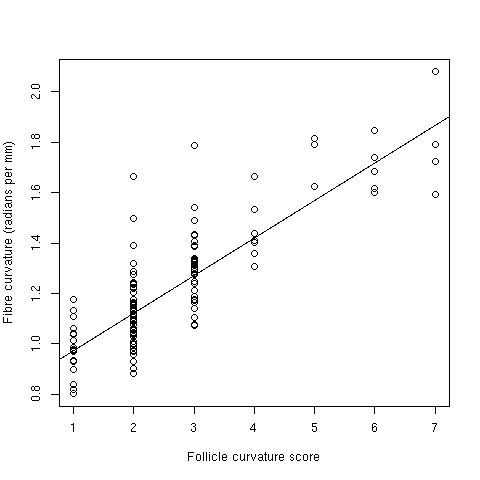
\includegraphics{ofdarads.png}
  \caption{Measured curvature of fibres in staples by OFDA technique for 159 sheep of   given follicle curvature score}
  \label{fig:ofdarads}
\end{figure}

%\end{document}



The fitted orthogonal regression equation was 

\begin{equation}
\label{eqn:in-staple}
Y = 0.8273 + 0.1481 X
\end{equation}

where Y is Fibre curvature (in radians per mm) and X is follicle curvature score.The fitted equation is shown as the straight line on Figure~\ref{fig:ofdarads}. The follicle curvature score and measured fibre curvature  had a correlation  of $0.821$.



The same data , with OFDA mean curvature expressed as fibre radius of curvature in mm are shown in Figure~\ref{fig:ofdamm}.

%\documentclass{article}
%\usepackage{graphicx,subfigure}
%\begin{document}

\begin{figure}[!h]
  \centering
   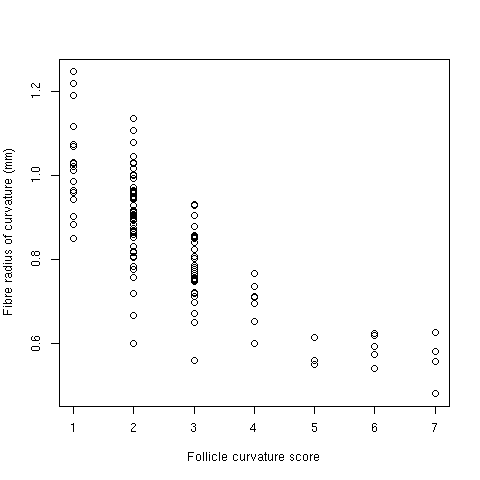
\includegraphics[width=0.9\textwidth]{ofdamm.png}
%  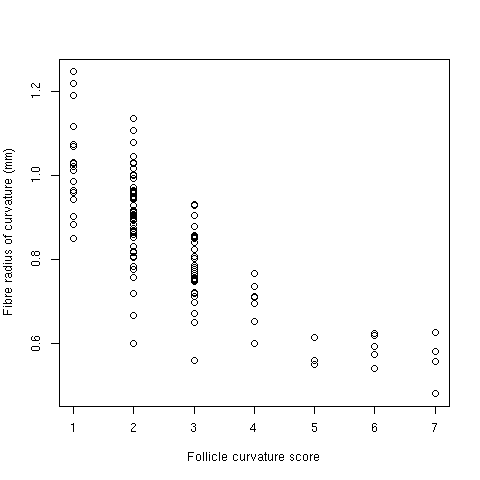
\includegraphics{ofdamm.png}
  \caption{Measured curvature of fibres in staples by OFDA technique expressed as radius of curvature in mm for 159 sheep of   given follicle curvature score}
  \label{fig:ofdamm}
\end{figure}

%\end{document}



This relationship is clearly nonlinear, as with the in-follicle data.

\subsection{Comparison of fibre curvature in follicles and in the staple}
So do we use equation~\ref{eqn:in-follicle} or ~\ref{eqn:in-staple} to predict intrinsic fibre curvature from follicle curvature? The two equations are not identical, so we need to look closely at the size and nature of their differences.

Figure~\ref{fig:ovly} shows the data and fitted regression lines from Figures~\ref{trandata} and ~\ref{fig:ofdarads} superimposed. The OFDA curvature data give a larger value for fibre curvature than the in-follicle measurements, especially at low follicle curvature scores. The difference is about 0.5 rads per mm at follicle curvature score 1, and it declines to about a zero difference at follicle curvature scores 5 and higher. 

%\documentclass{article}
%\usepackage{graphicx,subfigure}
%\begin{document}

\begin{figure}[!h]
  \centering
   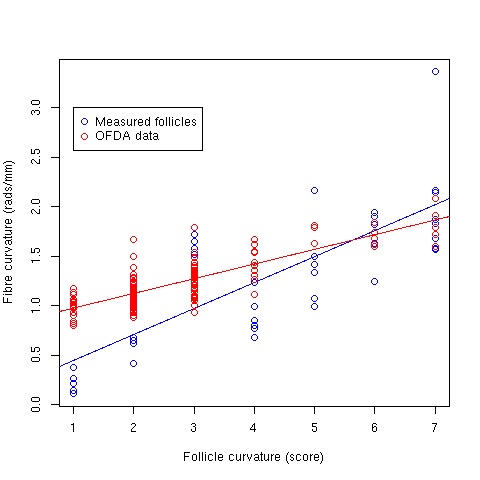
\includegraphics[width=0.9\textwidth]{ovly.png}
%  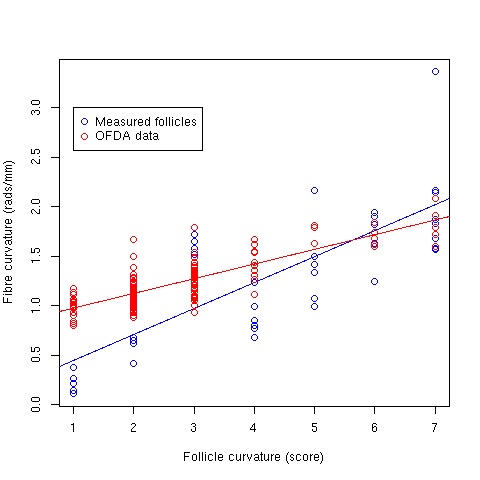
\includegraphics{ovly.png}
  \caption{Measured curvature of fibres in staples by OFDA technique for 159 sheep of   given follicle curvature score, superimposed on measured curvature of fibres in follicles. The two straight lines are orthogonal regression lines representing equations~\ref{eqn:in-follicle} and ~\ref{eqn:in-staple}.}
  \label{fig:ovly}
\end{figure}

%\end{document}



One can assume, on a stretched helix model of crimp, that fibres in a relaxed state ( ie exhibiting intrinsic fibre curvature) will have a lower curvature , because a relaxed helix is less curved ( larger radius) than a stretched helix. On this basis, we assert that the OFDA in staple measurements are not relaxed, at least for wools for which a stretched helix model is appropriate. We can correct for this, if we know the wavelength of the crimp, because the wavelength tells us how much the helix has been stretched. The formula is

\begin{equation}
\label{eqn:correct}
a_{c}^{2} = a_{s}^{2} + \left(\frac{\lambda}{2 \pi}\right)^{2}
\end{equation}

where $a_{c}$ is the radius of curvature of a compressed ( ie relaxed) helix, $a_{s}$ is the radius of curvature of a stretched helix, and $\lambda$ is the wavelength of the helix in the stretched state. 

Note that equation~\ref{eqn:correct} is for radius in mm, not curvature. To adjust the OFDA curvature data we need to calculate in several steps as follows
\begin{itemize}
\item change the OFDA curvature ( degrees per mm) to curvature in radians per mm using $C_{rads} = \pi C_{deg} / 180$
\item change from curvature to radius in mm using $R = 1/C_{rads}$
\item adjust the OFDA radius to intrinsic radius using equation~\ref{eqn:correct} $R_{adj} = \sqrt{R^{2} + \left(\frac{\lambda}{2 \pi}\right)_{2}}$
\item convert intrinsic radius to intrinsic curvature in radians per mm using $C_{adj} = 1 / R_{adj}$
\end{itemize}

We did all the above steps, for wools graded as "stretched" and "unaligned", but not for "unfolded" wools. The curvature of fibres in an "unfolded" wool staple is regarded as being at intrinsic radius of curvature ( except at the points whee fibres twist) and therefore does not require correction. We then fitted the orthogonal regression of the adjusted curvature on follicle curvature. Figure~\ref{fig:ovlyint} shows the data and fitted regression lines from Figure~\ref{trandata} and the the adjusted curvature data and its regression line, superimposed. 

%\documentclass{article}
%\usepackage{graphicx,subfigure}
%\begin{document}

\begin{figure}[!h]
  \centering
   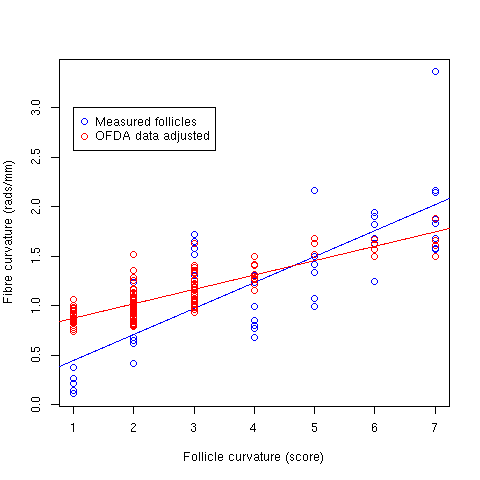
\includegraphics[width=0.9\textwidth]{ovlyint.png}
%  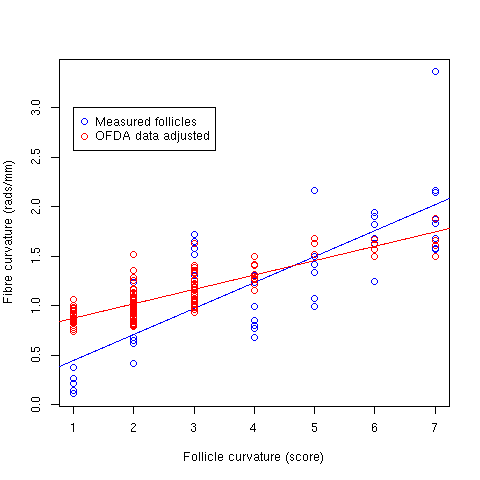
\includegraphics{ovlyint.png}
  \caption{Measured curvature of fibres in staples by OFDA technique for 159 sheep of   given follicle curvature score, superimposed on measured curvature of fibres in follicles. The OFDA mean curvture measurements for "stretched" and "unaligned" wools have been corrected to a relaxed state (intrinsic fibre curvature) assuming a stretched helix model for staple crimp. The two straight lines are orthogonal regression lines .}
  \label{fig:ovlyint}
\end{figure}

%\end{document}



Figure~\ref{fig:ovlyint} differs only a little from Figure~\ref{fig:ovly}. The adjustment has shifted the fibre curvatures down about 0.1 rads per mm, the new fitted equation being

\begin{displaymath}
Y = 0.7303 + 0.1442 * X
\end{displaymath}
 having a lower intercept and essentially the same slope.

So the adjusted OFDA curvatures are still larger than the in-follicle curvature measurements, and therefore the relationship to follicle curvature is slightly different. Most of the 159 wools in the OFDA-measured dataset would have an {\em unfolded} crimp rather than a {\em stretched} crimp. Correcting a curvature measurement from an {\em unfolded} wool back to a relaxed state is not as easy as for a wool with {\em stretched} helix crimp. An {\em unfolded} wool has two curvatures (Jackson and Watts(2016)~\cite{jack:16}).
\begin{itemize}
\item the bundle curvature which should be semicircular rather than sinusoidal, and which should be equal to intrinsic curvature because it is not stretched
\item the curvatures set in fibres by the twists at the points of inflection, which should have the radius of the twisted bundle of fibres ( approximately 0.1 mm but we have no precise figure)
\end{itemize}

So some curved sections of fibre from an {\em unfolded} wool will have intrinsic curvature, and some will have a high curvature ($1/0.1 = 10$ radians per mm) which is not intrinsic but is a {\em set} and may therefore fully or partly relax out depending on how the wool is treated. The distribution of in-staple curvtures should have a {\em tail} at the high end  due to the twisted parts of the fibres.

Calculating an adjustment to intrinsic curvature for {\em unfolded} wools is not feasible, there are too many assumptions in the above outline.

There is one other possibility, and that is that the in-follicle measurements of fibre curvature are biased downwards. This might happen if the follicles  were holding the fibres in a less curved state than would occur if the fibres were free. From personal observation of fibres emerging from follicles in vertical skin section, this is unlikely. The fibres are seen to emerge from the follicle in a continuous smooth curve which matches the curve of the follicles. There may be an orientation problem with the in-follicle measurments, but we would have expected that to be a bigger problem with high follicle curvature scores, and what we observe is a bigger discrepancy ( compared to OFDA curvature) with low follicle curvature scores.


\section{Discussion}
There is no way of knowing if prediction of intrinsic fibre curvature or radius from follicle curvature is biased, either in relation to Laserscan or OFDA measurements, or in relation to true intrinsic fibre curvature.

It is also entirely possible that  Laserscan of OFDA measurements are  themselves biased in relation to true intrinsic fibre curvature. The conditions of sample preparation in both these techniques are oriented toward fibre diameter measurement, and are not optimal for getting the fibre snippet into a properly relaxed condition for curvature measurement. To be fair, neither Laserscan or OFDA claim to measure intrinsic fibre curvature.

The conditions for measurement of intrinsic fibre curvature in the follicle in a vertical section are also probably not optimal for curvature measurement. In the live follicle the conditions are at least moist and may be stress free. In a vertical section which has been frozen, stained, and mounted in glycerine jelly, the effect on fibre curvature is simply unknown. 

There is no hope of a proper calibration against tedious single fibre measurement of intrinsic curvature under proper conditions. However the dual approach of predicting both in-follicle measurement of fibre curvature and OFDA measurement of fibre curvature gives us some credibility, even though the two techniques do not completely agree.

We have to make a decision. Which equation do we use for prediction of intrinsic fibre curvature from follicle curvature? At  the moment the indication is that we should stick with equation~\ref{eqn:in-follicle} developed from in-follicle measurements, at least for our purpose. For our purpose a slight bias is unlikely affect estimation of genetic parameters. We are only attempting to setup a linear transformation of follicle curvature, to get it into the correct units for use as intrinsic radius of curvature. A linear transform will not change a genetic analysis much. What may be affected are the traits we calculate from intrinsic radius as set out below.
 
The purpose behind developing this intrinsic fibre curvature prediction is to extend the scope of some genetic analyses of wool fibre and follicle characterisics. Most of the classic Merino genetics datasets have crimp frequency ($f$), and some have follicle curvature ($F_{c}$). If we can derive the intrinsic radius of curvature ($R$) from follicle curvature then we can also derive crimp wavelength ($\lambda$), crimp amplitude ($h$), and fibre length to staple length ratio ($L_{f}/L_{s}$). Given staple length ($L_{s}$) we can therefore get fibre length ($L_{f}$). The appropriate formulae, assuming a stretched helix crimp form, were derived by Jackson and Watts(2016)~\cite{jack:16}, and are as follows. 

\begin{eqnarray}
\lambda & = & \frac{25.4}{f} \\
h       & = & \sqrt{R^{2} - \left(\frac{\lambda}{2\pi}\right)^{2}} \\
\frac{L_{f}}{L_{s}} & = & \frac{2\pi R}{\lambda}\\
L_{f} & = & L_{s} \left(\frac{L_{f}}{L_{s}}\right)
\end{eqnarray}

There are a similar set of equations if one wishes to assume an unfolded helix, although this would probably not be a realistic assumption for the sheep in classic Merino genetics studies.

Given these derived traits it would be possible to obtain their genetic parameters and to include these important characteristics in a comprehensive multivariate analysis of genetic variation in wool and skin characteristics.

\begin{thebibliography}{99}

\bibitem{hori:53}
Horio, M. and Kondo, T. (1953) Text. Res. J. 23:373

\bibitem{jack:16}
Jackson, N. and Watts, J.E. (2016) Staple crimp formation in the fleece of Merino sheep. Unpublished manuscript, 18 May 2016.

\bibitem{nayj:73}
Nay, T. and Jackson, N. (1973) Effect of changes in nutritional level on the depth and curvature of wool follicles in Australian Merino sheep. Aust. J. Agric. Res. 24:439-447

\bibitem{onio:62}
Onions, W.J. (1962) Wool: an introduction to its properties, varieties, uses
     and production. Ernest Benn limited, London, 1962

\bibitem{rprog:13}
R Core Team (2013). R: A language and environment for statistical
  computing. R Foundation for Statistical Computing, Vienna, Austria.
  ISBN 3-900051-07-0, URL http://www.R-project.org/.

\bibitem{swan:93}
Swan, P.G. (1993) Objective measurement of fibre crimp curvature and the bulk compressional properties of Australian wools. PhD Thesis, University of NSW, March 1993 

\end{thebibliography}
\end{document}
